% Options for packages loaded elsewhere
\PassOptionsToPackage{unicode}{hyperref}
\PassOptionsToPackage{hyphens}{url}
%
\documentclass[
]{article}
\usepackage{amsmath,amssymb}
\usepackage{iftex}
\ifPDFTeX
  \usepackage[T1]{fontenc}
  \usepackage[utf8]{inputenc}
  \usepackage{textcomp} % provide euro and other symbols
\else % if luatex or xetex
  \usepackage{unicode-math} % this also loads fontspec
  \defaultfontfeatures{Scale=MatchLowercase}
  \defaultfontfeatures[\rmfamily]{Ligatures=TeX,Scale=1}
\fi
\usepackage{lmodern}
\ifPDFTeX\else
  % xetex/luatex font selection
\fi
% Use upquote if available, for straight quotes in verbatim environments
\IfFileExists{upquote.sty}{\usepackage{upquote}}{}
\IfFileExists{microtype.sty}{% use microtype if available
  \usepackage[]{microtype}
  \UseMicrotypeSet[protrusion]{basicmath} % disable protrusion for tt fonts
}{}
\makeatletter
\@ifundefined{KOMAClassName}{% if non-KOMA class
  \IfFileExists{parskip.sty}{%
    \usepackage{parskip}
  }{% else
    \setlength{\parindent}{0pt}
    \setlength{\parskip}{6pt plus 2pt minus 1pt}}
}{% if KOMA class
  \KOMAoptions{parskip=half}}
\makeatother
\usepackage{xcolor}
\usepackage[margin=1in]{geometry}
\usepackage{graphicx}
\makeatletter
\def\maxwidth{\ifdim\Gin@nat@width>\linewidth\linewidth\else\Gin@nat@width\fi}
\def\maxheight{\ifdim\Gin@nat@height>\textheight\textheight\else\Gin@nat@height\fi}
\makeatother
% Scale images if necessary, so that they will not overflow the page
% margins by default, and it is still possible to overwrite the defaults
% using explicit options in \includegraphics[width, height, ...]{}
\setkeys{Gin}{width=\maxwidth,height=\maxheight,keepaspectratio}
% Set default figure placement to htbp
\makeatletter
\def\fps@figure{htbp}
\makeatother
\setlength{\emergencystretch}{3em} % prevent overfull lines
\providecommand{\tightlist}{%
  \setlength{\itemsep}{0pt}\setlength{\parskip}{0pt}}
\setcounter{secnumdepth}{-\maxdimen} % remove section numbering
\newlength{\cslhangindent}
\setlength{\cslhangindent}{1.5em}
\newlength{\csllabelwidth}
\setlength{\csllabelwidth}{3em}
\newlength{\cslentryspacingunit} % times entry-spacing
\setlength{\cslentryspacingunit}{\parskip}
\newenvironment{CSLReferences}[2] % #1 hanging-ident, #2 entry spacing
 {% don't indent paragraphs
  \setlength{\parindent}{0pt}
  % turn on hanging indent if param 1 is 1
  \ifodd #1
  \let\oldpar\par
  \def\par{\hangindent=\cslhangindent\oldpar}
  \fi
  % set entry spacing
  \setlength{\parskip}{#2\cslentryspacingunit}
 }%
 {}
\usepackage{calc}
\newcommand{\CSLBlock}[1]{#1\hfill\break}
\newcommand{\CSLLeftMargin}[1]{\parbox[t]{\csllabelwidth}{#1}}
\newcommand{\CSLRightInline}[1]{\parbox[t]{\linewidth - \csllabelwidth}{#1}\break}
\newcommand{\CSLIndent}[1]{\hspace{\cslhangindent}#1}
\usepackage{setspace}\doublespacing
\ifLuaTeX
  \usepackage{selnolig}  % disable illegal ligatures
\fi
\IfFileExists{bookmark.sty}{\usepackage{bookmark}}{\usepackage{hyperref}}
\IfFileExists{xurl.sty}{\usepackage{xurl}}{} % add URL line breaks if available
\urlstyle{same}
\hypersetup{
  pdftitle={An Open-Source Application to Computerize Simple Market Efficiency Games},
  pdfauthor={James T. Bang},
  hidelinks,
  pdfcreator={LaTeX via pandoc}}

\title{An Open-Source Application to Computerize Simple Market
Efficiency Games}
\author{James T. Bang}
\date{15 Aug 2023}

\begin{document}
\maketitle
\begin{abstract}
In-class experiments provide instructors a powerful tool for helping
students learn and understand market principles in economics. Despite
the effectiveness of experiments, economics instructors remain slow to
adopt them in their pedagogy. One reason for this lag could be the
time-consuming process of collecting, tabulating, and presenting the
outcomes of the experiments. This paper introduces functions and
ShinyApps in R for fast, free, in-class tabulation of the results of
five in-class market simulation experiments for teaching economics.\\
\textbf{Keywords:} Experiments; technology; teaching\\
\textbf{JEL Code:} A22
\end{abstract}

\pagenumbering{gobble}
\newpage
\pagenumbering{arabic}
\setcounter{page}{1}

\hypertarget{introduction}{%
\section{Introduction}\label{introduction}}

The use of experiments as demonstrations of economic theory date back at
least as far as those conducted by Chamberlin (1948) and Smith (1962).
These studies were designed primarily to collect evidence supporting or
refuting economic models of rational behavior in market settings. Holt
(1993) summarizes this literature. While experiments remain an important
method for observing behavior to test economic hypotheses, these
experiments have also found their way into pedagogy (DeYoung 1993).

Classroom experiments offer students and instructors a fun departure
from the usual ``chalk and talk'' of explaining economic models. In
addition to entertainment value, studies have shown experiments to
increase student learning in post-test assessments (Emerson and Taylor
2004; Dickie 2006). I should note, however, that not all studies
conclude that all types of gamification improves learning by a
significant margin: Gremmen and Potters (1997) find a positive effect of
games on average, but the effect is not statistically significant, while
Dickie (2006) finds that games do significantly improve learning, but
that attaching grade incentives to the games do not contribute any
additional benefit. Moreover, Stodder (1998) expresses concern that
classroom games that penalize cooperation may teach and reinforce
unethical decision making.

Despite the potential learning and entertainment value of classroom
experiments, they remain relatively rare among the pedagogies economics
professors adopt in their classrooms (Watts and Becker 2008). Two
factors may drive some of the hesitancy among economics instructors to
implement classroom experiments. On the one hand, free resources, such
as those described in the survey of non-computerized games by Brauer and
Delemeester (2001), require significant time investments to tabulate and
summarize the results. On the other hand, automated resources,
especially those distributed by textbook publishers, impose a financial
cost on students or their institutions that instructors feel rightly
averse to asking budget-constrained students or departments to foot the
bill for.

Cheung (2008) helps to overcome this barrier by building tools for
collecting student responses to in-class non-computerized experiments
using mobile phones and texting. This contribution furthers this by
automating the process of calculating and summarizing the results of the
experiments. These examples only require students to be able to access a
Google Form via their browser on their computer or mobile device, which,
given the ubiquity of mobile phones among students (sometimes as their
only personal computing device), sets a fairly reasonable bar for
accessibility. A secondary contribution is simplifying existing versions
of classic market equilibrium, entry, and duopoly games with the hope of
increasing the diversity of methods used by economics instructors in the
classroom.

On the instructor's end, I have created a free, downloadable package
called \texttt{econGame} for the \emph{R} open-source statistical
computing program. The tabulation programs run as either stand-alone
functions in the \emph{R} console, or for demonstration purposes as a
html \emph{Shiny} app that can open in a browser tab if desired. This
allows the instructor to present the results of the experiment almost
instantaneously after the students have submitted their responses.

\hypertarget{description-of-the-experiments}{%
\section{Description of the
Experiments}\label{description-of-the-experiments}}

The models I will describe in this paper encompass two well-established
market equilibrium games known to the economics education literature
Brauer and Delemeester (2001), namely simplified versions of the
following experiments:\\
1. the pit market trading game introduced by Holt (1996);\\
2. the entry and exit game introduced by Garratt (2000); and three games
simulating different oligopoly models (Bertrand, Cournot, and
Stackelberg). In the examples the ``payoffs'' students receive can be
awarded to the students at the end of the games as ``extra credit''
points, or instructors may choose to encourage students to play the
games strategically, but only ``for the love of the game.'' I briefly
describe the delivery of the games below.

\hypertarget{pit-market-trading}{%
\subsection{Pit Market Trading}\label{pit-market-trading}}

Holt (1996) designed the pit market trading game for class sizes between
10 and 25 and takes about 40-50 minutes to explain the game, play a few
rounds, and tabulate the results after each round. This game is an
excellent illustration of supply and demand, competitive market
equilibrium, consumer and producer surplus, and efficiency. The
functions presented in this paper speed up the response-collection
process to allow the experiment to work for larger classes. It also
speeds up the calculation of the equilibrium and graphs the equilibrium.

Before class, the instructor prepares (1) a Google Sheet assigning a
random integer between 1 and 10 representing each student's value that
they place on the asset;\footnote{The first sheet consists of a single
  formula in a single cell: ``=roundup(10*rand())``. A template can be
  found at:\\
  \url{https://docs.google.com/spreadsheets/d/1lCmC692ajsQZoatWtgZh5QKaJ9y3pOMt15JwRFaHanU/edit\#gid=258904023}.}
and (2) a Google Form through which students enter their bid and ask
prices;\footnote{A template can be found at:\\
  \url{https://docs.google.com/forms/d/1S_F9UJ6GXttxPqDLtk8Hg0ZgzDaHMxBmc1qH3W2gKZo/edit}.}
For the best compatibility with the result-tabulating function, users
who create their own forms should use the question prompts ``First
Name,'' ``Last Name'', ``Round,'' ``Value,'' ``Bid,'' and ``Ask.'' Add
text fields to insert additional context, instructions, or question
text.

In class, the instructor informs the students that they own a single
unit of an asset that each of them values differently. This value could
represent a profit that they can derive from using the asset as a
resource to produce other goods, a return the students expect to receive
from selling the asset in the future, or a subjective ``utility'' that
the students derive from using the asset as consumption. Students
discover this value by visiting a link to the first Google Sheet that
the instructor prepared to assign a random value from 1 to 10.

Students submit their name, the round number (if playing more than one),
their randomly-assigned value draw, a ``bid'' corresponding to the
highest amount they would pay for a second unit of the asset, and an
``ask'' corresponding to the lowest amount they would accept to part
with the unit of the asset they already own.

If the instructor decides to incentivize the game with points, students
keep their consumer and producer surpluses from each round as ``extra
credit'' points. \texttt{equilibriumGame} tabulates the supply and
demand schedules; calculates the equilibrium; graphs the equilibrium;
and tabulates the scores for each student.\footnote{The solution the
  piece-wise constant supply and demand equilibrium uses the help of a
  C++ helper function provided by ``David'' on Stack Overflow,\\
  \url{https://stackoverflow.com/questions/23830906/intersection-of-two-step-functions}.}

\hypertarget{entry-and-exit}{%
\subsection{Entry and Exit}\label{entry-and-exit}}

Garratt (2000) designed an entry and exit game with four discrete
specifications of the demand functions for class sizes between 25 and
44. Garratt's version also includes four markets (corn, wheat, rice, and
soybeans), while the one presented here only includes two (corn and
soybeans). The demand functions in this version of the experiment
automatically adjust according to the number of students participating.
Garratt's version of the game also takes about 45 minutes to complete
the experiment (including a government ``fallow program'' intervention
variation), usually about five rounds.

Before class the instructor prepares a Form to collect responses that
includes the fields ``First Name,'' ``Last Name,'' ``Round,'' and
``Market.''\footnote{A template can be found at:\\
  \url{https://docs.google.com/forms/d/1oUsLulfD5bqT6_9VVYIzLWuuQ-L4vwmC4jI-1jabOVQ/edit}.}
Other information that might be useful to add to the Form includes
information about demand and costs in each sector. The default inverse
demand functions allow for each market to reward producers with about
one unit of ``normal profit,'' but these settings can be changed.

In class, the instructor informs the students that they will choose to
plant corn, soybeans, or nothing. Producing corn incurs a cost of four,
while producing soybeans incurs a cost of 10. Garratt (2000) recommends
that the instructor \emph{not} reveal the demand functions to students,
whereas some instructors (including me) might prefer to allow students
to play with perfect information. Selling a unit of corn brings revenue
equal to \(P_c = (N/2) + 6 - Q_c\), where \(N\) equals the number of
students participating and \(Q_c\) equals the number of students
choosing to produce corn. Selling a unit of soybeans brings revenue
equal to \(P_s = (N/2) + 10 - Q_s\). These parameters allow for there to
be a ``normal profit'' of about one unit per student in each market in
equilibrium, to compensate for the risk of venturing into
self-employment.\footnote{The long run equilibrium, with 1 unit of
  ``normal profit'' occurs with \((N/2) + 1\) students choosing corn and
  \((N/2) - 1\) students choosing soybeans.} If the instructor wants the
prices to equal whole numbers (and the profits to equalize), they can
join the game as a ``student'' to round out the numbers.

If the instructor decides to play the game with points, students earn
points equal to their profits. Students may play as many rounds as the
instructor decides to continue the game, or until the markets reach the
long run equilibrium of zero \emph{economic} profit. Usually the markets
converge to the long run equilibrium by the end of about five rounds.
Padding the demand functions to leave one point of ``normal profit''
compared to sitting out simulates the concept of a normal profit
business owners receive for taking risk and lessens the chances that
students might ``win'' negative extra credit points. Students choosing
to produce nothing sell their labor in the labor market and earn zero
(they do not earn a normal profit).

\hypertarget{oligoply-models}{%
\subsection{Oligoply Models}\label{oligoply-models}}

I also constructed a set of games to demonstrate and compare equilibria
in different (two-firm) oligopoly models. In each of the examples,
students work in pairs. The instructor informs the students that the
market price depends on both the strategy they choose for their ``firm''
and also the strategy their partner chooses. Each of the three examples
uses the following linear inverse demand function (the parameters of
which individual instructors may change in the options):
\(P = a + b(Q_1 + Q_2),\) where the default values for the parameters
are \(a = 10\) and \(b = -1\). Likewise, firms face the the same cost
function: \(TC = f + cQ_i,\) where \(f\) represents the fixed cost (0 by
default) and \(c\) represents the (constant) marginal (and average) cost
of each additional unit (6 by default).

Before beginning any of the duopoly models, the instructor should solve
the competitive and monopoly equilibria with students first so that
students can see the plausible range of prices they should expect to
declare. Skipping this step often leads to a few greedy (but
quantitatively-challenged) students choosing prices that would result in
negative quantities. With the default parameters, the competitive
equilibrium price and quantity are 6 and 4, while the monopoly
equilibrium price and quantity are 8 and 2.

\hypertarget{bertrand-duoploy}{%
\subsubsection{Bertrand Duoploy}\label{bertrand-duoploy}}

Before class, the instructor prepares the Form to collect the responses,
which includes the fields ``First Name,'' ``Last Name'', ``Partner First
Name,'' ``Partner Last Name,'' ``Round,'' and ``Price.''\footnote{A
  template can be found at:\\
  \url{https://docs.google.com/forms/d/1AykOoY6mVj17D_5CW7-BLhSgOJdGEhyfYHKHROnvdcg/edit}.}
The package also includes a function to assign partners randomly using
the class roster (saved as a Google Sheet), and the
\texttt{bertrandGame()} function even allows the instructor to randomize
the partners \emph{after the fact} in case the instructor really wants
to cut down on tacit collusion. The package default calculates the
results using student-entered partners.

In class, the instructor reviews the competitive and monopoly equilibria
for the demand function in the example. The instructor then presents the
``rules'' for the Bertrand model as a ``winner takes all'' market.
Students submit their own names, partner's names, and their price. \[
Q_1 = \begin{cases}
    0 & \text{if } P_1 > P_2 \\ 
    (10 - P_1)/2 & \text{if } P_1 = P_2 \\
    10 - P_1 & \text{if } P_1 < P_2 
\end{cases}
\] If the instructor chooses to use points for the activity, students
earn points equal to their profit.

\hypertarget{cournot-duopoly}{%
\subsubsection{Cournot Duopoly}\label{cournot-duopoly}}

Before class, the instructor prepares the Form to collect the responses,
which includes the fields ``First Name,'' ``Last Name'', ``Partner First
Name,'' ``Partner Last Name,'' ``Round,'' and ``Strategy''\footnote{A
  template can be found at:\\
  \url{https://docs.google.com/forms/d/1dp-tUv5rNhRpm9UjFCy_pgsD4rJJnja-QJnWnMu81DI/edit}.}
As with the Bertrand game, instructors have discretion over allowing
students to choose their own partners (``rivals'') or randomizing the
partners before or after the students choose a strategy.

In the Cournot game, students choose either to ``collude'' (produce a
low quantity) or ``defect'' (produce a high quantity). The function that
tabulates the results assigns half of the monopolist's profit-maximizing
quantity to students who choose ``collude,'' and automatically assigns
the quantity corresponding to the best response function for students
who choose ``defect'' (which depends on the output choice of their
rival). Students only need to make the simple binary choice. Instructors
using this example for upper-level classes may (or may not) want to edit
the game settings to require students to submit a specific quantity
(derive the best response functions themselves).

\hypertarget{stackelberg-duopoly}{%
\subsubsection{Stackelberg Duopoly}\label{stackelberg-duopoly}}

Similar to the Cournot game, students in the Stackelberg game choose to
``collude'' or ``defect.'' In contrast to the Cournot game, students
must know their partner in advance, and followers will see the leaders'
strategy choices before choosing their strategy. The function again
automatically calculates the quantities corresponding to the set of
binary strategy choices to determine the payoff outcomes.{[}\^{}A
template can be found at:\\
\url{https://docs.google.com/forms/d/1vERPMPt_kW96JPAY6mEtkQMu6FLCgPuqoFL8i8bulYk/edit}.{]}

\hypertarget{the-econgame-package}{%
\section{The econGame Package}\label{the-econgame-package}}

The \texttt{econGame} package pulls activity data from Google the Google
Sheet file generated for the form responses. It then tabulates, scores,
and graphs the responses; and writes the grade data to a separate Google
Sheet. Users can download the package from
\url{https://github.com/bangecon/econGame}. To install the package, use
the \texttt{remotes} package and the \texttt{install\_github()}
function:

\texttt{remotes::install\_github("bangecon/econGame")}

\hypertarget{exporting-the-results}{%
\subsection{Exporting the Results}\label{exporting-the-results}}

Once the students have completed each round of a game, the instructor
should pause to tabulate the results for that round. This is especially
the case in the entry and exit game, where convergence to the long-run
equilibrium requires students to know which sector earned economic
profits in the previous round. To do this, the instructor needs to click
the Google Sheets icon in the responses tab of the edit page of the
form. Figure 1 demonstrates where to find these tools in your Google
Form.

\begin{figure}
\centering
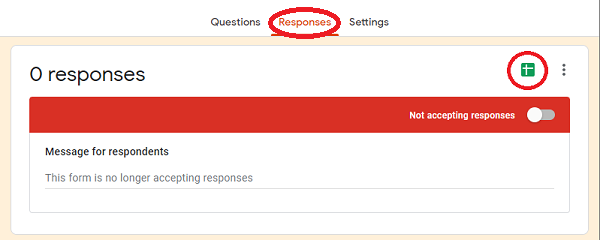
\includegraphics{images/Figure1.png}
\caption{Exporting Results to Google Sheets}
\end{figure}

This creates a Google Sheet that contains all of the data for tabulating
the results.\footnote{Link the Form to a Sheet to collect responses by
  selecting the ``Responses'' tab, and clicking ``Link to Sheets.''}

In order to link to your results, you will need to copy to your
clipboard the sheet ID from the URL. Figure 2 shows where you can find
the sheet ID for your results.

\begin{figure}
\centering
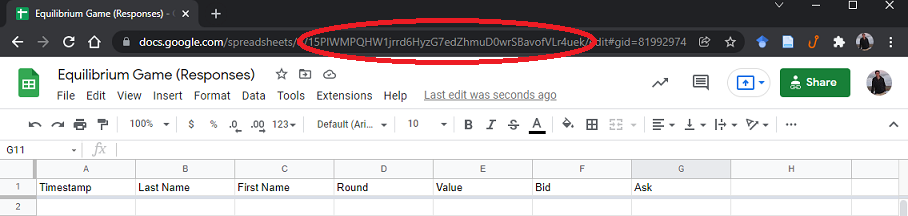
\includegraphics{images/Figure2.png}
\caption{Finding the Sheet ID}
\end{figure}

\hypertarget{tabulating-the-results}{%
\subsection{Tabulating the Results}\label{tabulating-the-results}}

Each game has its own function to tabulate its results, and for each
function there are slightly different options that the instructor can
adjust based on any changes they might have made to the default
parameters for the exercise. The only argument the instructor needs to
provide (and that does not have a preset default) is the ID of the
Google Sheet. The syntax and outputs for the different functions are:

\begin{itemize}
\item
  Equilibrium game: \texttt{equilibriumGame(sheet\ =\ NULL,\ ...)}

  \begin{itemize}
  \item
    Arguments:

    \begin{itemize}
    \tightlist
    \item
      \texttt{sheet} (required) is a character string url corresponding
      to the Google Sheets location containing the individual
      submissions.
    \end{itemize}
  \item
    Outputs:

    \begin{itemize}
    \tightlist
    \item
      \texttt{type} returns the type of activity (equlibriumGame).
    \item
      \texttt{results} returns the original submissions (with market
      price and points added).
    \item
      \texttt{schedules} returns a list containing the supply and demand
      schedules for each round.
    \item
      \texttt{equilibria} returns a list containing the equilibria for
      each round.
    \item
      \texttt{grades} returns the aggregated points ``won'' by each
      student for the entire activity.
    \end{itemize}
  \end{itemize}
\item
  Entry and exit game: \texttt{entryGame(sheet\ =\ NULL,\ ...)}

  \begin{itemize}
  \item
    Arguments:

    \begin{itemize}
    \tightlist
    \item
      \texttt{sheet} (required) is a character string url corresponding
      to the Google Sheets location containing the individual
      submissions.
    \end{itemize}
  \item
    Outputs:

    \begin{itemize}
    \tightlist
    \item
      \texttt{type} returns the type of activity (equlibriumGame).
    \item
      \texttt{results} returns the original submissions (with market
      price and points added).
    \item
      \texttt{rounds} returns the number of rounds in ``results.''
    \item
      \texttt{equilibria} returns a list containing the equilibria for
      each round.
    \item
      \texttt{grades} returns the aggregated points ``won'' by each
      student for the entire activity.
    \end{itemize}
  \end{itemize}
\item
  Bertrand game:
  \texttt{bertrandGame(sheet\ =\ NULL,\ a\ =\ 10,\ b\ =\ -1,\ c\ =\ 6,\ f\ =\ 0,\ ...)}

  \begin{itemize}
  \item
    Arguments:

    \begin{itemize}
    \tightlist
    \item
      \texttt{sheet} (required) is a character string url corresponding
      to the Google Sheets location containing the individual
      submissions.
    \item
      \texttt{a} is the value of the intercept of the linear
      inverse-demand function (default is 10).
    \item
      \texttt{b} is the value of the slope of the linear inverse-demand
      function (default is -1).
    \item
      \texttt{c} is the value of the firm's marginal cost (default is
      6).
    \item
      \texttt{f} is the value of the firm's fixed cost (default is 0).
    \end{itemize}
  \item
    Outputs:

    \begin{itemize}
    \tightlist
    \item
      \texttt{type} returns the type of activity (equlibriumGame).
    \item
      \texttt{results} returns the original submissions (with market
      price and points added).
    \item
      \texttt{grades} returns the aggregated points ``won'' by each
      student for the entire activity.
    \end{itemize}
  \end{itemize}
\item
  Cournot game:
  \texttt{cournotGame(sheet\ =\ NULL,\ a\ =\ 10,\ b\ =\ -1,\ c\ =\ 6,\ f\ =\ 0,\ ...)}

  \begin{itemize}
  \item
    Arguments:

    \begin{itemize}
    \tightlist
    \item
      \texttt{sheet} (required) is a character string url corresponding
      to the Google Sheets location containing the individual
      submissions.
    \item
      \texttt{a} is the value of the intercept of the linear
      inverse-demand function (default is 10).
    \item
      \texttt{b} is the value of the slope of the linear inverse-demand
      function (default is -1).
    \item
      \texttt{c} is the value of the firm's marginal cost (default is
      6).
    \item
      \texttt{f} is the value of the firm's fixed cost (default is 0).
    \end{itemize}
  \item
    Outputs:

    \begin{itemize}
    \tightlist
    \item
      \texttt{type} returns the type of activity (equlibriumGame).
    \item
      \texttt{results} returns the original submissions (with market
      price and points added).
    \item
      \texttt{grades} returns the aggregated points ``won'' by each
      student for the entire activity.
    \end{itemize}
  \end{itemize}
\item
  Stackelberg game:
  \texttt{stackelbergGame(sheet\ =\ NULL,\ a\ =\ 10,\ b\ =\ -1,\ c\ =\ 6,\ f\ =\ 0,\ ...)}

  \begin{itemize}
  \item
    Arguments:

    \begin{itemize}
    \tightlist
    \item
      \texttt{sheet} (required) is a character string url corresponding
      to the Google Sheets location containing the individual
      submissions.
    \item
      \texttt{a} is the value of the intercept of the linear
      inverse-demand function (default is 10).
    \item
      \texttt{b} is the value of the slope of the linear inverse-demand
      function (default is -1).
    \item
      \texttt{c} is the value of the firm's marginal cost (default is
      6).
    \item
      \texttt{f} is the value of the firm's fixed cost (default is 0).
    \end{itemize}
  \item
    Outputs:

    \begin{itemize}
    \tightlist
    \item
      \texttt{type} returns the type of activity (equlibriumGame).
    \item
      \texttt{results} returns the original submissions (with market
      price and points added).
    \item
      \texttt{grades} returns the aggregated points ``won'' by each
      student for the entire activity.
    \end{itemize}
  \end{itemize}
\end{itemize}

Another feature of the package is the ability to plot the results. The
syntax to plot any of the games described in this paper is simply
\texttt{plot(econGame,\ ...)}, where the (sole) argument is the name of
an object assigned by one of the \texttt{econGame} functions. The plot
the function generates depends on the type of game:

\begin{itemize}
\tightlist
\item
  For
  \texttt{type\ =\ \textquotesingle{}equilibriumGame\textquotesingle{}},
  plot the supply and demand functions with the corresponding equlibrium
  point.
\item
  For \texttt{type\ =\ \textquotesingle{}entryGame\textquotesingle{}},
  plot the supply, demand, and per-unit cost lines to show profits and
  losses.
\item
  For
  \texttt{type\ =\ \textquotesingle{}bertrandGame\textquotesingle{}},
  plot a histogram of the price strategies.
\item
  For \texttt{type\ =\ \textquotesingle{}cournotGame\textquotesingle{}}
  or
  \texttt{type\ =\ \textquotesingle{}stackelbergGame\textquotesingle{}},
  plot a bar graph of the strategy outcomes.
\end{itemize}

\hypertarget{shiny-user-interface}{%
\subsection{Shiny User Interface}\label{shiny-user-interface}}

The functions for directly summarizing the results of the games may be
useful for tabulating the results for the purposes of awarding points to
the students who participated, but may not be the most
visually-appealing way to present the results in class. To improve the
user interface for a ``prettier'' presentation of the results, I have
built a Shiny Application UI for each of the games. In this interface,
the instructor can display the raw results, plots, or schedules of the
outcomes of the results by inputting the sheet ID (and other parameters)
in the input boxes, and by switching the display tabs of the results.

To run the Shiny App for a given package, I have written a function that
executes the app from the
\texttt{\textquotesingle{}\textasciitilde{}/inst/shiny-examples\textquotesingle{}}
folder of the package source. Once the instructor has installed the
package, all they need to do to execute the app is type one of the
following commands:
\texttt{\textquotesingle{}runEquilibriumGameApp()\textquotesingle{}},
\texttt{\textquotesingle{}runEntryGameApp()\textquotesingle{}},
\texttt{\textquotesingle{}runBertrandGameApp()\textquotesingle{}},
\texttt{\textquotesingle{}runCournotGameApp()\textquotesingle{}}, or
\texttt{\textquotesingle{}runStackelbergGameApp()\textquotesingle{}}.
When the instructor initiates the app, it will point the function to a
blank Google Sheet as the default, which will result in either blank
output, or an error. In order to read the submission results, the
instructor will need to paste the Google Sheet ID depicted in Figure 2.

Figure 3 shows the Shiny interface for \texttt{equilibriumGame}. Within
the output panel, the instructor (and students) will be able to see
tabbed output for different results, plots, and possibly the grade
outcomes if the instructor wishes to show it.

\begin{figure}
\centering
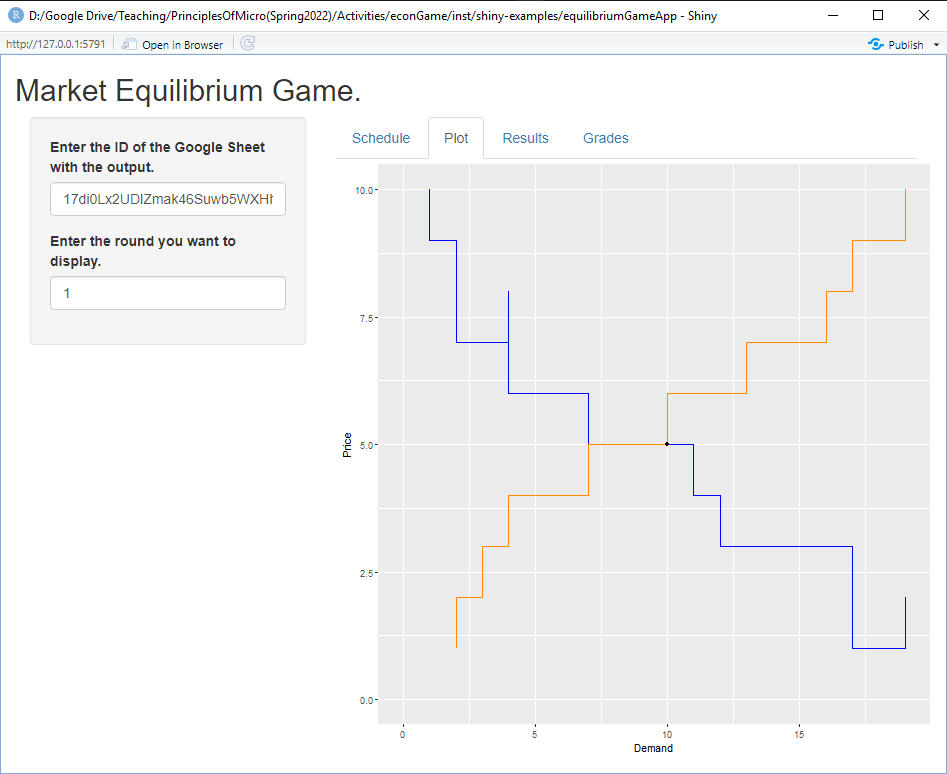
\includegraphics{images/Figure3.png}
\caption{Shiny User Interface}
\end{figure}

\hypertarget{discussion}{%
\section{Discussion}\label{discussion}}

This work provided examples of how to implement some simple market games
using R and Shiny. The objective of the functions developed for this
discussion was to help instructors adopt more creative and engaging
teaching methods in their principles classrooms by lowering both the
financial and time costs of tabulating the results and presenting
appealing summaries of the outcomes.

All of the examples can be implemented for the students using Google
Forms, which collects the results in Google Sheets. Instructors may then
tabulate the results using the \texttt{econGame} package via the HTML
Shiny App with a single-function command in R. All of these applications
and packages come at no cost to the student. The only potential cost
barrier is the device - which could be as little as a mobile device -
each student would need in order to input their responses.

Another useful feature is that I have platformed the package on GitHub,
which allows users to make pull requests to suggest edits and changes to
improve or add features and examples to the package. I plan to also
develop more functions and applications for the \texttt{econGame}
package from existing classroom experiments, and even design a few
original games. If you use these resources, please let me know and share
them with your colleagues.

\hypertarget{references}{%
\section*{References}\label{references}}
\addcontentsline{toc}{section}{References}

\hypertarget{refs}{}
\begin{CSLReferences}{1}{0}
\leavevmode\vadjust pre{\hypertarget{ref-brauer_games_2001}{}}%
Brauer, Jurgen, and Greg Delemeester. 2001. {``Games Economists Play:
{A} Survey of Non-Computerized Classroom-Games for College Economics.''}
\emph{Journal of Economic Surveys} 15 (2): 221--36.

\leavevmode\vadjust pre{\hypertarget{ref-chamberlin_experimental_1948}{}}%
Chamberlin, Edward H. 1948. {``An Experimental Imperfect Market.''}
\emph{Journal of Political Economy} 56 (2): 95--108.

\leavevmode\vadjust pre{\hypertarget{ref-cheung_using_2008}{}}%
Cheung, Stephen L. 2008. {``Using {Mobile} {Phone} {Messaging} as a
{Response} {Medium} in {Classroom} {Experiments}.''} \emph{The Journal
of Economic Education} 39 (1): 51--67.
\url{https://doi.org/10.3200/JECE.39.1.51-67}.

\leavevmode\vadjust pre{\hypertarget{ref-deyoung_market_1993}{}}%
DeYoung, Robert. 1993. {``Market Experiments: {The} Laboratory Versus
the Classroom.''} \emph{The Journal of Economic Education} 24 (4):
335--51.

\leavevmode\vadjust pre{\hypertarget{ref-dickie_classroom_2006}{}}%
Dickie, Mark. 2006. {``Do {Classroom} {Experiments} {Increase}
{Learning} in {Introductory} {Microeconomics}?''} \emph{The Journal of
Economic Education} 37 (3): 267--88.
\url{https://doi.org/10.3200/JECE.37.3.267-288}.

\leavevmode\vadjust pre{\hypertarget{ref-emerson_comparing_2004}{}}%
Emerson, Tisha LN, and Beck A. Taylor. 2004. {``Comparing Student
Achievement Across Experimental and Lecture-Oriented Sections of a
Principles of Microeconomics Course.''} \emph{Southern Economic
Journal}, 672--93.

\leavevmode\vadjust pre{\hypertarget{ref-garratt_free_2000}{}}%
Garratt, Rod. 2000. {``A Free Entry and Exit Experiment.''}
\emph{Journal of Economic Education} 31 (3): 237.
\url{https://www.proquest.com/docview/235237213/citation/8DF4FB2251DE443BPQ/1}.

\leavevmode\vadjust pre{\hypertarget{ref-gremmen_assessing_1997}{}}%
Gremmen, Hans, and Jan Potters. 1997. {``Assessing the Efficacy of
Gaming in Economic Education.''} \emph{The Journal of Economic
Education} 28 (4): 291--303.

\leavevmode\vadjust pre{\hypertarget{ref-holt_industrial_1993}{}}%
Holt, Charles A. 1993. {``Industrial {Organization}: {A} {Survey} of
{Laboratory} {Research}.''}

\leavevmode\vadjust pre{\hypertarget{ref-holt_classroom_1996}{}}%
---------. 1996. {``Classroom Games: {Trading} in a Pit Market.''}
\emph{Journal of Economic Perspectives} 10 (1): 193--203.

\leavevmode\vadjust pre{\hypertarget{ref-smith_experimental_1962}{}}%
Smith, Vernon L. 1962. {``An Experimental Study of Competitive Market
Behavior.''} \emph{Journal of Political Economy} 70 (2): 111--37.

\leavevmode\vadjust pre{\hypertarget{ref-stodder_experimental_1998}{}}%
Stodder, James. 1998. {``Experimental Moralities: {Ethics} in Classroom
Experiments.''} \emph{The Journal of Economic Education} 29 (2):
127--38.

\leavevmode\vadjust pre{\hypertarget{ref-watts_little_2008}{}}%
Watts, Michael, and William E. Becker. 2008. {``A {Little} {More} Than
{Chalk} and {Talk}: {Results} from a {Third} {National} {Survey} of
{Teaching} {Methods} in {Undergraduate} {Economics} {Courses}.''}
\emph{The Journal of Economic Education} 39 (3): 273--86.
\url{https://doi.org/10.3200/JECE.39.3.273-286}.

\leavevmode\vadjust pre{\hypertarget{ref-williams_economic_1993}{}}%
Williams, Arlington W., and James M. Walker. 1993. {``Economic
{Instruction} {Computerized} {Laboratory} {Exercises} for
{Microeconomics} {Education}: {Three} {Applications} {Motivated} by
{Experimental} {Economics}.''} \emph{Journal of Economic Education
(1986-1998)} 24 (4): 291.
\url{https://www.proquest.com/docview/216514673/abstract/C674FBF2453242F6PQ/1}.

\end{CSLReferences}

\end{document}
